%% AMS-LaTeX Created with the Wolfram Language for Students - Personal Use Only : www.wolfram.com

\documentclass{article}
\usepackage{amsmath, amssymb, graphics, setspace}

\newcommand{\mathsym}[1]{{}}
\newcommand{\unicode}[1]{{}}

\newcounter{mathematicapage}
\begin{document}

I.1 \(x-\text{$\pi $y}+\sqrt[3]{5}z=0\) is a linear equation\\
I.2 \(x^2+y^2+z^2=1\) is NOT a linear equation\\
I.3 \(x^{-1}+7y+z=\)\(\left(\text{Sin}\left[\frac{\pi }{9}\right]\right)^2\) is NOT a linear equation\\
I.4 \(x+7y+z=\text{Sin}\left[\frac{\pi }{9}\right]\) is a linear equation\\
I.5 \(3\text{Cos}[x]-4y+z=\sqrt{3}\) is NOT a linear equation\\
I.6 \(\text{Cos}[3]x-4y+z=\sqrt{3}\) is a linear equation

II.7

\begin{doublespace}
\noindent\(\pmb{\text{ContourPlot}[\{x + y \text{==} 0, 2*x + y \text{==} 3\}, \{x, 2, 4\}, \{y, -4, -2\},\text{ContourStyle}\to \{\text{Blue},\text{Orange}\}]}\\
\pmb{\text{(*}}\\
\pmb{
\begin{array}{ll}
 \{ & 
\begin{array}{ll}
 x+y & =0 \\
 2x+y & =3 \\
\end{array}
 \\
\end{array}
\Rightarrow \left(
\begin{array}{ccc}
 1 & 1 & 0 \\
 2 & 1 & 3 \\
\end{array}
\right)\Rightarrow R_2-2R_1\Rightarrow \left(
\begin{array}{ccc}
 1 & 1 & 0 \\
 0 & -1 & 3 \\
\end{array}
\right)\Rightarrow 
\begin{array}{ll}
 \{ & 
\begin{array}{ll}
 x+y & =0 \\
 -y & =3 \\
\end{array}
 \\
\end{array}
}\\
\pmb{y=-3}\\
\pmb{}\\
\pmb{x+y=0}\\
\pmb{x=-(-3)}\\
\pmb{x=3}\\
\pmb{\text{*)}}\\
\pmb{\text{Solve}[\{x + y \text{==} 0,2*x + y \text{==} 3\}, \{x,y\}]}\)
\end{doublespace}

\includegraphics{HWork02_linear_eqs_gr1.eps}

\begin{doublespace}
\noindent\(\{\{x\to 3,y\to -3\}\}\)
\end{doublespace}

II.8

\begin{doublespace}
\noindent\(\pmb{\text{ContourPlot}[\{x - 2*y \text{==} 7, 3*x + y \text{==} 7\}, \{x, 2, 4\}, \{y, -3, -1\},\text{ContourStyle}\to \{\text{Blue},\text{Orange}\}]}\\
\pmb{\text{(*}}\\
\pmb{
\begin{array}{ll}
 \{ & 
\begin{array}{ll}
 x-2y & =7 \\
 3x+y & =7 \\
\end{array}
 \\
\end{array}
\Rightarrow \left(
\begin{array}{ccc}
 1 & -2 & 7 \\
 3 & 1 & 7 \\
\end{array}
\right)\Rightarrow R_2-3R_1\Rightarrow \left(
\begin{array}{ccc}
 1 & -2 & 7 \\
 0 & 7 & -14 \\
\end{array}
\right)\Rightarrow 
\begin{array}{ll}
 \{ & 
\begin{array}{ll}
 x-2y & =7 \\
 7y & =-14 \\
\end{array}
 \\
\end{array}
}\\
\pmb{y=-2}\\
\pmb{}\\
\pmb{x-2y=7}\\
\pmb{x=7+2(-2)}\\
\pmb{x=3}\\
\pmb{\text{*)}}\\
\pmb{\text{Solve}[\{x - 2*y \text{==} 7,3*x + y \text{==} 7\}, \{x,y\}]}\)
\end{doublespace}

\includegraphics{HWork02_linear_eqs_gr2.eps}

\begin{doublespace}
\noindent\(\{\{x\to 3,y\to -2\}\}\)
\end{doublespace}

II.9

\begin{doublespace}
\noindent\(\pmb{\text{ContourPlot}[\{3*x - 6*y \text{==} 3, -x + 2*y \text{==} 1\}, \{x, -3.125, 4.5\}, \{y, -1.75, 1.75\},\text{ContourStyle}\to
\{\text{Blue},\text{Orange}\}]}\\
\pmb{\text{(*}}\\
\pmb{
\begin{array}{ll}
 \{ & 
\begin{array}{ll}
 3x-6y & =3 \\
 -x+2y & =1 \\
\end{array}
 \\
\end{array}
\Rightarrow \left(
\begin{array}{ccc}
 3 & -6 & 3 \\
 -1 & 2 & 1 \\
\end{array}
\right)\Rightarrow R_2+\frac{1}{3}R_1\Rightarrow \left(
\begin{array}{ccc}
 3 & -6 & 3 \\
 0 & 0 & 2 \\
\end{array}
\right)\Rightarrow 
\begin{array}{ll}
 \{ & 
\begin{array}{ll}
 3x-6y & =3 \\
 0 & =2 \\
\end{array}
 \\
\end{array}
}\\
\pmb{\text{no} \text{solution}}\\
\pmb{\text{*)}}\\
\pmb{\text{Solve}[\{ 3*x - 6*y \text{==} 3,\text{  }-x + 2*y \text{==} 1\}, \{x,y\}]}\)
\end{doublespace}

\includegraphics{HWork02_linear_eqs_gr3.eps}

\begin{doublespace}
\noindent\(\{\}\)
\end{doublespace}

\begin{doublespace}
\noindent\(\pmb{\text{VIII}}\\
\pmb{
\begin{array}{ll}
 \{ & 
\begin{array}{ll}
 \text{kx}+y & =-2 \\
 2x-2y & =4 \\
\end{array}
 \\
\end{array}
\Rightarrow \left(
\begin{array}{ccc}
 k & 1 & -2 \\
 2 & -2 & 4 \\
\end{array}
\right)\Rightarrow \frac{1}{k}R_1\Rightarrow \left(
\begin{array}{ccc}
 1 & \frac{1}{k} & -\frac{2}{k} \\
 2 & -2 & 4 \\
\end{array}
\right)\Rightarrow R_2-2R_1\Rightarrow \left(
\begin{array}{ccc}
 1 & \frac{1}{k} & -\frac{2}{k} \\
 0 & -\frac{2 (1+k)}{k} & 4+\frac{4}{k} \\
\end{array}
\right)\Rightarrow -\frac{k}{2 (1+k)}R_2\Rightarrow \left(
\begin{array}{ccc}
 1 & \frac{1}{k} & -\frac{2}{k} \\
 0 & 1 & -2 \\
\end{array}
\right)\Rightarrow R_1-\frac{1}{k}R_2\Rightarrow \left(
\begin{array}{ccc}
 1 & 0 & 0 \\
 0 & 1 & -2 \\
\end{array}
\right)}\\
\pmb{
\begin{array}{c}
 x=0 \\
 y=-2; \text{for} \text{all} k \\
\end{array}
}\)
\end{doublespace}

\begin{doublespace}
\noindent\(\pmb{A=\left(
\begin{array}{ccc}
 k & 1 & -2 \\
 2 & -2 & 4 \\
\end{array}
\right);}\\
\pmb{\text{RowReduce}[A];}\\
\pmb{\text{MatrixForm}[\%]}\\
\pmb{\text{Solve}[\{k*x+y==-2,2x-2y==4\},\{x,y\}]}\\
\pmb{\text{xMin}=-3;}\\
\pmb{\text{xMax}=2;}\\
\pmb{\text{ContourPlot3D}[\{k*x+y==-2,2x-2y==4\},\{x,\text{xMin},\text{xMax}\},\{y,\text{xMin},\text{xMax}\},\{k,\text{xMin},\text{xMax}\},\text{Axes}\to
\text{True},\text{AxesLabel}\to \{x,y,z\},}\\
\pmb{\text{PlotLegends}\to \text{{``}Expressions{''}}]}\)
\end{doublespace}

\begin{doublespace}
\noindent\(\left(
\begin{array}{ccc}
 1 & 0 & 0 \\
 0 & 1 & -2 \\
\end{array}
\right)\)
\end{doublespace}

\begin{doublespace}
\noindent\(\{\{x\to 0,y\to -2\}\}\)
\end{doublespace}

\begin{doublespace}
\noindent\(\begin{array}{cc}
  &  \\
\end{array}\)
\end{doublespace}

Optional 1\\
Consider the following matrix\\
A=\(\left(
\begin{array}{ccc}
 \pi  & \pi  & \pi  \\
 \pi ^2 & \pi ^2 & \pi ^2 \\
 \pi ^3 & \pi ^3 & \pi ^3 \\
\end{array}
\right)\)\\
1. Find the reduced row echelon from of A; then find the rank of A.\\
2. How can you enter in Mathenatica (in one line) the matrix A? (without typing every entry!). Hint: Consider the Table command.\\
3. Now generalize the result as follows: let X be the following arbitrary square matrix of size n, where c is any non-zero number. Compute the rank
of X.\\
X=\(\left(
\begin{array}{cccc}
 c & c & \cdots  & c \\
 c^2 & c^2 & \cdots  & c^2 \\
 \vdots  & \vdots  & \vdots  & \vdots  \\
 c^n & c^n & \cdots  & c^n \\
\end{array}
\right)\)

Optional 1.1

\begin{doublespace}
\noindent\(\pmb{A=;}\\
\pmb{\text{Print}[\text{{``}RowReduce[A]={''}} \text{MatrixForm}[\text{RowReduce}[A]]]}\\
\pmb{\text{Print}[\text{{``}MatrixRank[A]={''}}]}\\
\pmb{\text{MatrixRank}[A]}\)
\end{doublespace}

\noindent\(\text{RowReduce[A]=} \left(
\begin{array}{ccc}
 1 & 1 & 1 \\
 0 & 0 & 0 \\
 0 & 0 & 0 \\
\end{array}
\right)\)

\noindent\(\text{MatrixRank[A]=}\)

\begin{doublespace}
\noindent\(1\)
\end{doublespace}

Optional 1.2

\begin{doublespace}
\noindent\(\pmb{A=\text{Table}[\text{Pi}{}^{\wedge}i,\{i,1,3\},\{j,1,3\}];}\\
\pmb{\text{MatrixForm}[A]}\)
\end{doublespace}

\begin{doublespace}
\noindent\(\left(
\begin{array}{ccc}
 \pi  & \pi  & \pi  \\
 \pi ^2 & \pi ^2 & \pi ^2 \\
 \pi ^3 & \pi ^3 & \pi ^3 \\
\end{array}
\right)\)
\end{doublespace}

Optional 1.3\\
X=\(\left(
\begin{array}{cccc}
 c & c & \cdots  & c \\
 c^2 & c^2 & \cdots  & c^2 \\
 \vdots  & \vdots  & \vdots  & \vdots  \\
 c^n & c^n & \cdots  & c^n \\
\end{array}
\right)\Rightarrow\) \(\begin{array}{c}
 \frac{1}{X_{11}}R_1\rightarrow R_1 \\
 \frac{1}{X_{21}}R_2\rightarrow R_2 \\
 \vdots  \\
 \frac{1}{X_{\text{n1}}}R_n\rightarrow R_n \\
\end{array}
\Rightarrow\) \(\left(
\begin{array}{cccc}
 1 & 1 & \cdots  & 1 \\
 1 & 1 & \cdots  & 1 \\
 \vdots  & \vdots  & \vdots  & \vdots  \\
 1 & 1 & \cdots  & 1 \\
\end{array}
\right)\Rightarrow\) \(\begin{array}{c}
 R_2-R_1\rightarrow R_2 \\
 R_3-R_1\rightarrow R_3 \\
 \vdots  \\
 R_n-R_1\rightarrow R_n \\
\end{array}
\Rightarrow\) \(\left(
\begin{array}{cccc}
 1 & 1 & \cdots  & 1 \\
 0 & 0 & \cdots  & 0 \\
 \vdots  & \vdots  & \vdots  & \vdots  \\
 0 & 0 & \cdots  & 0 \\
\end{array}
\right)\)

Optional 2\\
For what value(s) of k, if any, will the following system:\\
\(\begin{array}{ll}
 \{ & 
\begin{array}{ll}
 x+y+\text{kz} & =1 \\
 x+\text{ky}+z & =1 \\
 \text{kx}+y+z & =-2 \\
\end{array}
 \\
\end{array}\)\\
have\\
1. No solution\\
2. A unique solution\\
3. Infinitely many solutions\\
Hint. Find the reduced echelon form of the augmented matrix, then analyze different cases (beware of division by zero!).\\
\\
\(\begin{array}{ll}
 \{ & 
\begin{array}{ll}
 x+y+\text{kz} & =1 \\
 x+\text{ky}+z & =1 \\
 \text{kx}+y+z & =-2 \\
\end{array}
 \\
\end{array}
\Rightarrow\) \(\left(
\begin{array}{cccc}
 1 & 1 & k & 1 \\
 1 & k & 1 & 1 \\
 k & 1 & 1 & -2 \\
\end{array}
\right)\Rightarrow\) \(R_1\leftrightarrow R_3\Rightarrow\) \(\left(
\begin{array}{cccc}
 k & 1 & 1 & -2 \\
 1 & k & 1 & 1 \\
 1 & 1 & k & 1 \\
\end{array}
\right)\Rightarrow\) \(\frac{1}{k}R_1\rightarrow R_1\Rightarrow\) \(\left(
\begin{array}{cccc}
 1 & \frac{1}{k} & \frac{1}{k} & -\frac{2}{k} \\
 1 & k & 1 & 1 \\
 1 & 1 & k & 1 \\
\end{array}
\right)\Rightarrow\) \(\begin{array}{c}
 R_2-R_1\rightarrow R_2 \\
 R_3-R_1\rightarrow R_3 \\
\end{array}
\Rightarrow\) \(\left(
\begin{array}{cccc}
 1 & \frac{1}{k} & \frac{1}{k} & -\frac{2}{k} \\
 0 & k-\frac{1}{k} & 1-\frac{1}{k} & 1+\frac{2}{k} \\
 0 & 1-\frac{1}{k} & k-\frac{1}{k} & 1+\frac{2}{k} \\
\end{array}
\right)\Rightarrow\) \(R_1-\frac{1}{-1+k^2}R_2\rightarrow R_1\Rightarrow\) \(\left(
\begin{array}{cccc}
 1 & 0 & \frac{1}{1+k} & \frac{1+2k}{1-k^2} \\
 0 & k-\frac{1}{k} & 1-\frac{1}{k} & 1+\frac{2}{k} \\
 0 & 1-\frac{1}{k} & k-\frac{1}{k} & 1+\frac{2}{k} \\
\end{array}
\right)\Rightarrow\) \(\frac{k}{-1+k^2}R_2\rightarrow R_2\Rightarrow\) \(\left(
\begin{array}{cccc}
 1 & 0 & \frac{1}{1+k} & \frac{1+2k}{1-k^2} \\
 0 & 1 & \frac{1}{1+k} & \frac{2+k}{-1+k^2} \\
 0 & 1-\frac{1}{k} & k-\frac{1}{k} & 1+\frac{2}{k} \\
\end{array}
\right)\Rightarrow\) \(R_3-\left(1-\frac{1}{k}\right)R_2\rightarrow R_3\Rightarrow\) \(\left(
\begin{array}{cccc}
 1 & 0 & \frac{1}{1+k} & \frac{1+2k}{1-k^2} \\
 0 & 1 & \frac{1}{1+k} & \frac{2+k}{-1+k^2} \\
 0 & 0 & k-\frac{2}{1+k} & 1+\frac{1}{1+k} \\
\end{array}
\right)\Rightarrow\) \(\frac{1+k}{-2+k+k^2}R_3\rightarrow R_3\Rightarrow\) \(\left(
\begin{array}{cccc}
 1 & 0 & \frac{1}{1+k} & \frac{1+2k}{1-k^2} \\
 0 & 1 & \frac{1}{1+k} & \frac{2+k}{-1+k^2} \\
 0 & 0 & 1 & \frac{1}{-1+k} \\
\end{array}
\right)\Rightarrow\) \(\begin{array}{c}
 R_2-\frac{1}{1+k}R_3\rightarrow R_2 \\
 R_1-\frac{1}{1+k}R_3\rightarrow R_1 \\
\end{array}
\Rightarrow\) \(\left(
\begin{array}{cccc}
 1 & 0 & 0 & -\frac{2}{-1+k} \\
 0 & 1 & 0 & \frac{1}{-1+k} \\
 0 & 0 & 1 & \frac{1}{-1+k} \\
\end{array}
\right)\)\\
\(\begin{array}{c}
 
\begin{array}{c}
 z=\frac{1}{-1+k} \\
 y=\frac{1}{-1+k} \\
\end{array}
 \\
 x=-\frac{2}{-1+k} \\
\end{array}\)

Optional 2.1\\
The system does not have a solution for k = 1.

Optional 2.2 $\&$ 2.3\\
Since y = z, the system does not have a unique solution. Therefore the system has infinitely many solutions for k $\neq $ 1.

\begin{doublespace}
\noindent\(\pmb{A=\left(
\begin{array}{cccc}
 1 & 1 & k & 1 \\
 1 & k & 1 & 1 \\
 k & 1 & 1 & -2 \\
\end{array}
\right);}\\
\pmb{\text{RowReduce}[A];}\\
\pmb{\text{MatrixForm}[\%]}\\
\pmb{\text{Solve}[\{x+y+k*z==1,x+k*y+z==1,k*x+y+z==-2\},\{x,y,z\}]}\)
\end{doublespace}

\begin{doublespace}
\noindent\(\left(
\begin{array}{cccc}
 1 & 0 & 0 & -\frac{2}{-1+k} \\
 0 & 1 & 0 & \frac{1}{-1+k} \\
 0 & 0 & 1 & \frac{1}{-1+k} \\
\end{array}
\right)\)
\end{doublespace}

\begin{doublespace}
\noindent\(\left\{\left\{x\to -\frac{2}{-1+k},y\to \frac{1}{-1+k},z\to \frac{1}{-1+k}\right\}\right\}\)
\end{doublespace}

\end{document}
